\newpage


\chapter{ Guía de Usuario}
\label{chap:manual-usuario}

RobotUI es una aplicación web creada con un claro propósito; el de  proporcionar a los usuarios un medio donde compartir sus dispositivos robóticos con el resto de usuarios.\\

Para ello RobotUI proporciona una serie de herramientas para que, aquellas personas que no tengan los suficientes conocimientos de programación, puedan configurar un
entorno para el manejo de sus proyectos robóticos y tener posibilidad de compartir sus experiencias con el resto de usuarios.\\

La particularidad de RobotUI es que el usuario propietario del robot tiene la posibilidad de permitir el manejo de sus dispositivos robóticos al resto de usuarios que él mismo considere de una 
manera controlada o, por otra parte, permitir que otros usuarios visualicen, como si de espectadores se tratase, el control que un determinado usuario realiza de un determinado robot.
Todo ello en tiempo real.\\

Por tanto, tras esta breve introducción en el ámbito de la aplicación, en este manual se describen los diferentes paso a realizar para configurar sus dispositivos correctamente en el sistema
y abrirlo a toda una comunidad de usuarios. Además de tener abierto el acceso a otros muchos dispositivos de otras personas.\\

\subsection{Objetivo de esta guía}

Esta guía tiene como objetivo proporcionar al usuario un soporte de ayuda e iniciación a la utilización de RobotUI.\\

Esta sección comprende:\\

\begin{itemize}
 \item Guía de acceso al código fuente de la aplicación.
 \item Guía de uso de la aplicación.
 \item Guía para la puesta en marcha y programación de un robot.
\end{itemize}

\subsection{Dirigido a}

Esta guía esta dirigida al usuario final del proyecto RobotUI. Tiene la finalidad de proporcionar una guía descriptiva de los procedimientos de creación, configuración y utilización de los diferentes dispositivos 
robóticos en sus dos modalidades disponibles, la de control y la de visualización.

\subsection{Obtener RobotUI}

El código fuente junto con la presente memoria se encuentra disponible en el repositorio GitHub en el enlace \url{https://github.com/lopi87/SAILS-RobotUI} o usando la herramienta
Git, escribiendo en la consola el siguiente comando:\\

\begin{lstlisting}[language=bash]
 git clone git@github.com:lopi87/SAILS-RobotUI.git 
\end{lstlisting}


\section{ Uso de RobotUI }
\label{sec:uso-robotui}


\subsection{ Acceso a la aplicación }
\label{sec:acceso-aplicacion}

Para acceder a la aplicación, el usuario deberá accedes al siguiente enlace: \url{www.robotui.com}. \\

Al dar clic en la url podrá ver el portal de entrada a la aplicación, desde donde puede acceder a la aplicación con sus credenciales y/o  acceder a los formularios de \emph{registro de usuario}.

\begin{figure}[H]
  \begin{center}
    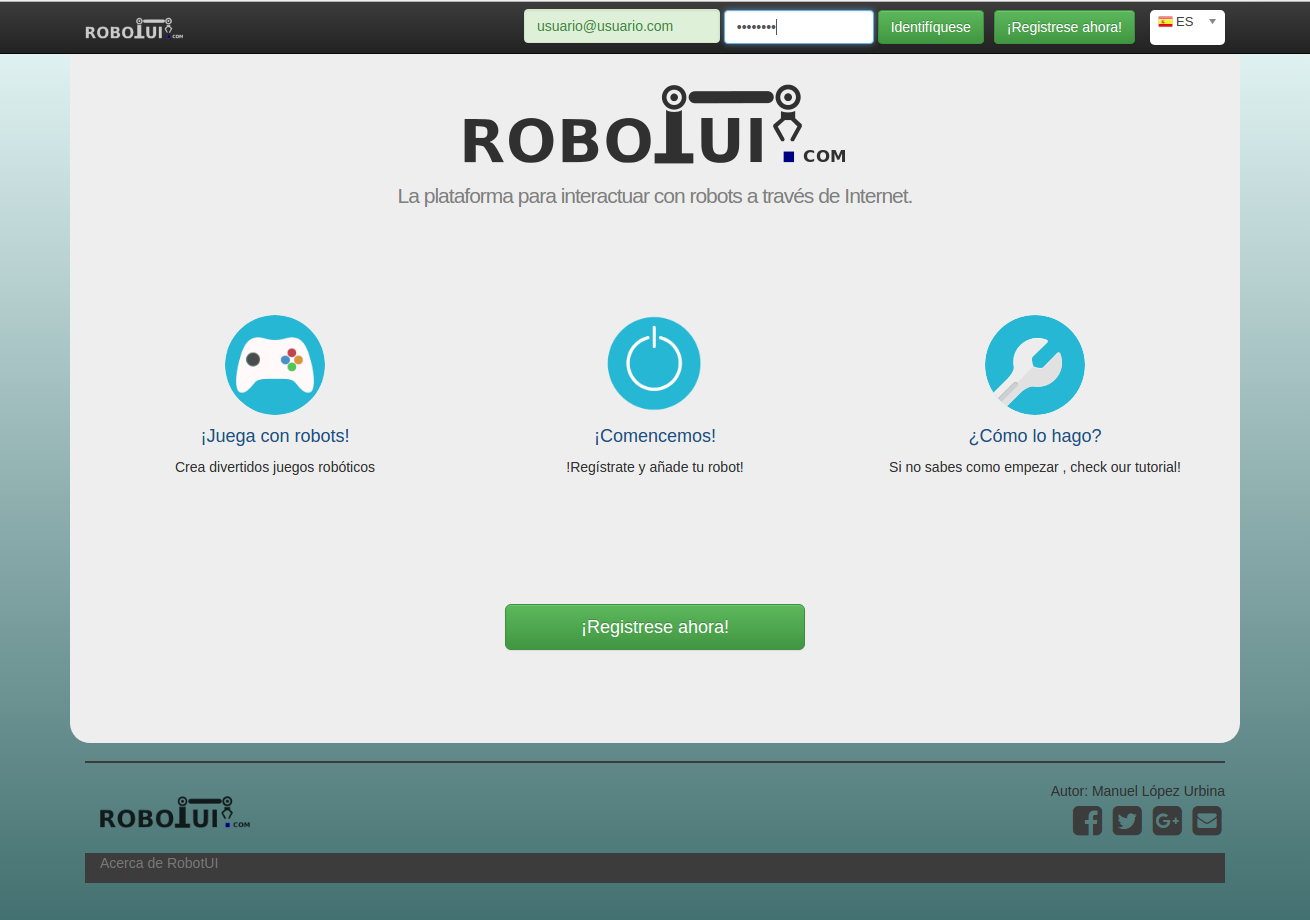
\includegraphics[scale=0.3]{imagenes/manual-usuario/pagina-principal.png}
  \end{center}
  \caption{Página principal RobotUI.}
  \label{website:pagina-principal}
\end{figure}


\subsection{ Registo de usuario }
\label{sec:creacion-usuario}


Una vez en la página principal, figura \ref{website:pagina-principal}, podemos observar la barra superior, la cual posee dos estados, la de usuario sin identificar y la de usuario identificado.


\begin{figure}[H]
  \begin{center}
    
\includegraphics[scale=0.5]{imagenes/manual-usuario/barra-menu1.png}
  \end{center}
  \caption{Vista de la barra superior en modalidad usuario no identificado en el sistema.}
  \label{website:pagina-principal}
\end{figure}

\begin{figure}[H]
  \begin{center}
    
\includegraphics[scale=0.5]{imagenes/manual-usuario/barra-menu2.png}
  \end{center}
  \caption{Vista de la barra superior en modalidad usuario identificado en el sistema.}
  \label{website:pagina-principal}
\end{figure}



Para iniciar el proceso de registro de usuario hacemos clic sobre el botón de la barra superior \emph{¡Regístrese ahora!} mediante el cual accedemos al formulario \ref{website:formulario-registro}.

\begin{figure}[H]
  \begin{center}
    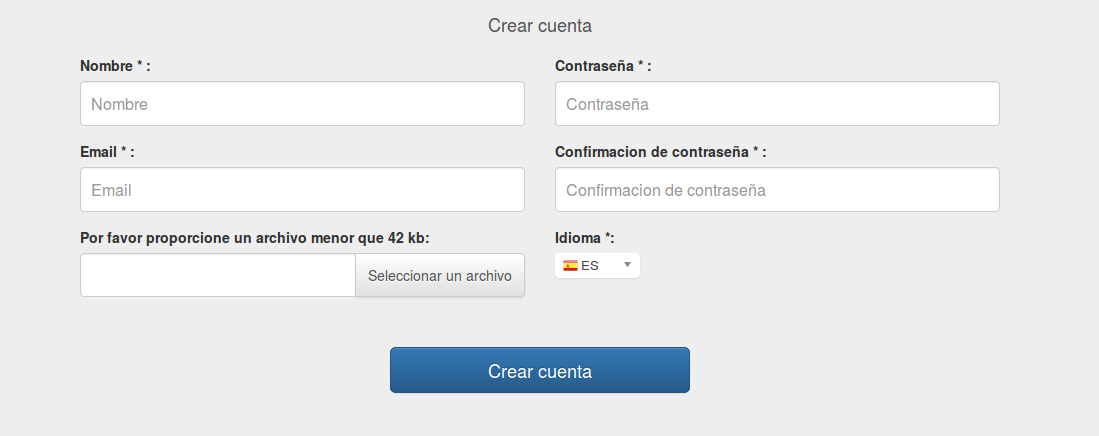
\includegraphics[scale=0.4]{imagenes/manual-usuario/pagina-registro.png}
  \end{center}
  \caption{Formulario de registro de usuario.}
  \label{website:formulario-registro}
\end{figure}

Para proceder con el registro necesitaremos los siguientes datos:

\begin{enumerate}
 \item Nombre: nombre de usuario.
 \item Email: dirección de correo electrónico utilizada para acceder al sistema.
 \item Contraseña: deberá proporcionar una contraseña para poder acceder al sistema.
 \item Confirmación de contraseña: campo para comprobar que la contraseña es la deseada por el usuario.
 \item Imagen: imagen avatar del usuario.
 \item Idioma: selección del idioma por defecto del usuario.
\end{enumerate}

Una vez introducidos los datos correctamente podremos hacer clic en \emph{crear cuenta}. Si los datos introducidos son correctos dispondremos de un nuevo usuario en la aplicación redirigiéndonos
a la página de información del nuevo usuario \ref{website:informacion-usuario}.

\begin{figure}[H]
  \begin{center}
    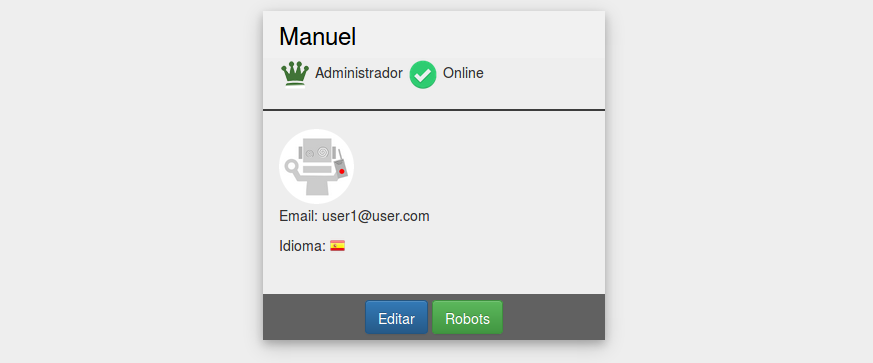
\includegraphics[scale=0.4]{imagenes/manual-usuario/informacion-usuario.png}
  \end{center}
  \caption{Información de un usuario.}
  \label{website:informacion-usuario}
\end{figure}


\subsection{Registro de un Robot}
\label{sec:creacion-robot}

Para el proceso de creación de un robot hacemos clic al menú \emph{Robots} \textrightarrow \enspace \emph{Mis robots} accediendo al formulario de creación, figura \ref{}.\\

En este caso registraremos nuestro robot de pruebas descrito en el capítulo \ref{chap:robot}. Para ello introducimos los siguientes datos:

\begin{enumerate}
 \item Nombre: nombre de nuestro robot.
 \item Dirección IP: dirección donde se encontrará accesible nuestro robot.
 \item Puerto: puerto donde se encontrará nuestro robot a la escucha de conexiones.
 \item Descripción: campo opcional en el que podemos añadir una descripción de nuestro robot y que será visible al resto de usuarios.
 \item Imagen: campo opcional en el que podremos subir una imagen de nuestro robot.
 \item Usuarios espectadores: selector en el que podemos especificar qué usuarios del sistema tendrán permisos para visualizar el funcionamiento de nuestro robot.
 \item Usuarios controladores: selector para especificar qué usuarios podrán tomar control de nuestro robot.
 \item Público: checkboxes para indicar si por el contrario, el robot que abierto a todos los usuarios para su control o abierto para su visualización si marcamos el primero o el segundo checkbox respectivamente
 y haciendo por tanto inválidos los parámetros de los selectores anteriores.
\end{enumerate}

Una vez rellenado los campos como se muestran en la imagen \ref{website:creacion-robot} pulsamos en \icontext{.2}{.35}{imagenes/manual-usuario/btn-crear.png}.

\begin{figure}[H]
  \begin{center}
    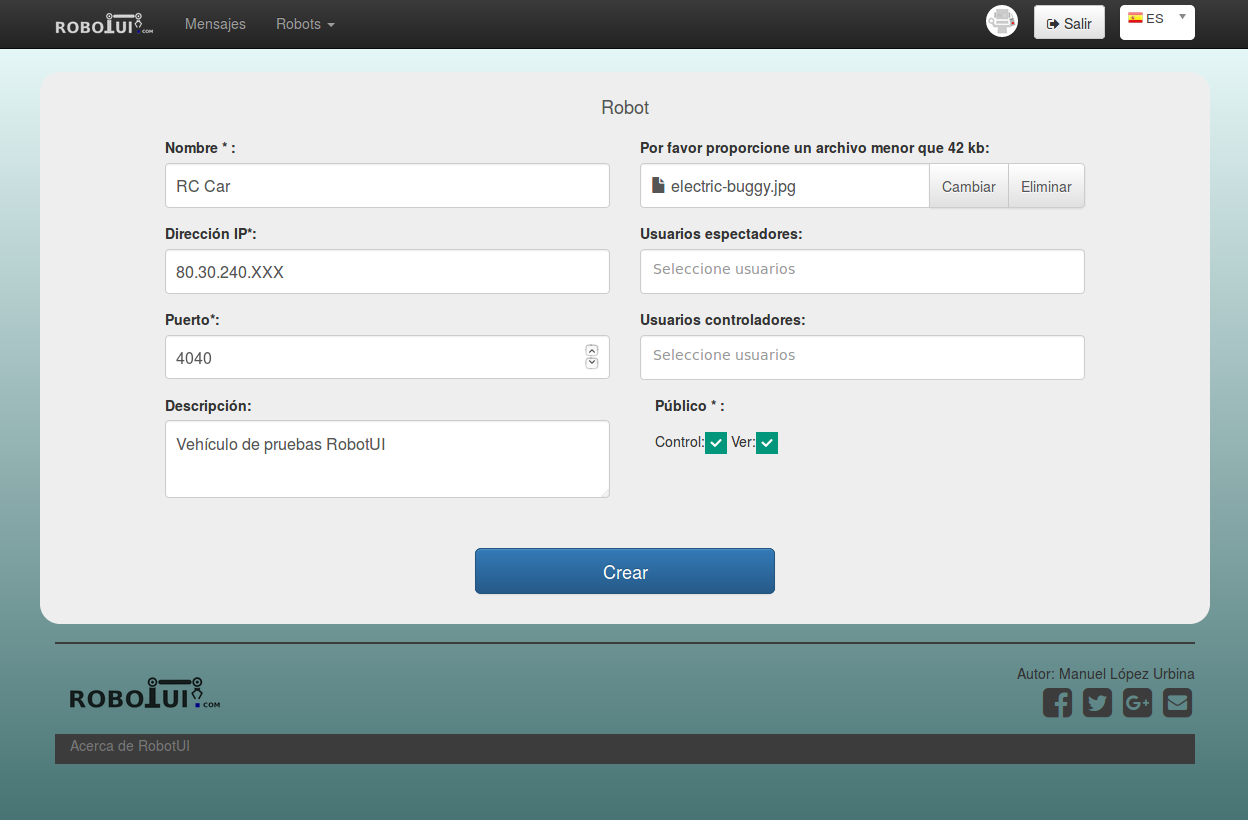
\includegraphics[scale=0.3]{imagenes/manual-usuario/pagina-crear-robot.png}
  \end{center}
  \caption{Formulario de creación de un robot.}
  \label{website:creacion-robot}
\end{figure}


Si los campos se han introducido correctamente visualizaremos la siguiente página:

\begin{figure}[H]
  \begin{center}
    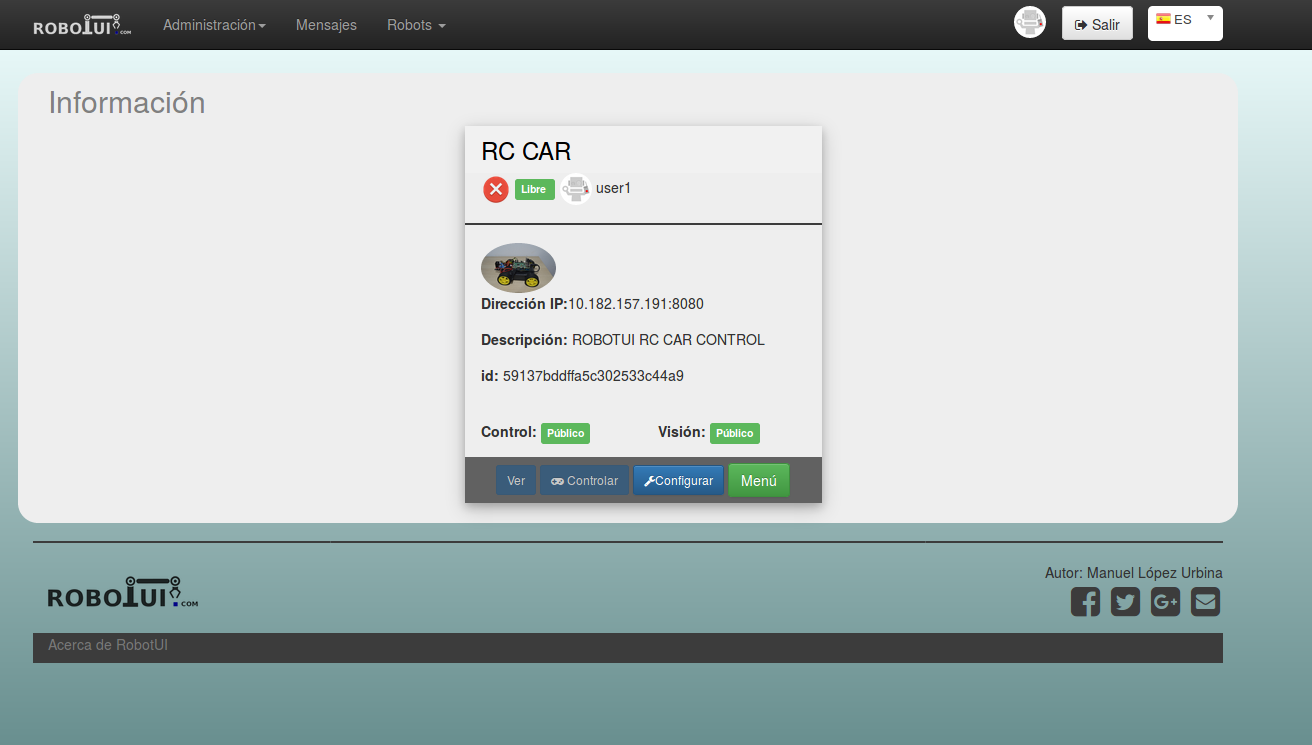
\includegraphics[scale=0.3]{imagenes/manual-usuario/show-robot.png}
  \end{center}
  \caption{Vista informativa de un robot.}
  \label{website:creacion-robot}
\end{figure}

En esta vista podemos apreciar la siguiente información:



\begin{table}[H]
  \begin{center}
    \begin{tabular}{|p{2cm}|p{10cm}|}
      \hline
      \centering{Elemento} & \qquad \quad Significado \\
      \hline
      
\includegraphics[width=1cm]{imagenes/manual-usuario/offline.png} & Imagen indicativa de que el robot se encuentra apagado. \\
      \hline
      
\includegraphics[width=1cm]{imagenes/manual-usuario/online.png} & Imagen indicativa de que el robot se encuentra encendido, reemplazará a la imagen apagado. \\
      \hline
      
\includegraphics[width=2cm]{imagenes/manual-usuario/control-publico.png} & Imagen representativa de que un robot es de control público. \\
      \hline
      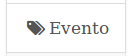
\includegraphics[width=1cm]{imagenes/manual-usuario/nuevo-evento.png} & Imagen representativa de que un robot es de control privado. \\
      \hline
      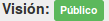
\includegraphics[width=2cm]{imagenes/manual-usuario/vision-publico.png} & Imagen representativa de que un robot es de visualización pública. \\
      \hline
      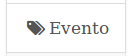
\includegraphics[width=1cm]{imagenes/manual-usuario/nuevo-evento.png} & Imagen representativa de que un robot es de visualización privada. \\
      \hline
    \end{tabular}
  \end{center}
\caption{Elementos de una interfaz.}
\end{table}





\subsection{Configuración de la interfaz}

Una vez creado nuestro robot en el sistema ya podemos configurar su interfaz. En la figura \ref{website:configuracion-interfaz} podemos ver el canvas sobre el que iremos añadiendo los diferentes elementos que 
conformarán nuestro panel de control. Esta interfaz servirá además de para controlar el dispositivo como ventana de seguimiento a los usuarios que visiten el funcionamiento del dispositivo.

\begin{figure}[H]
  \begin{center}
    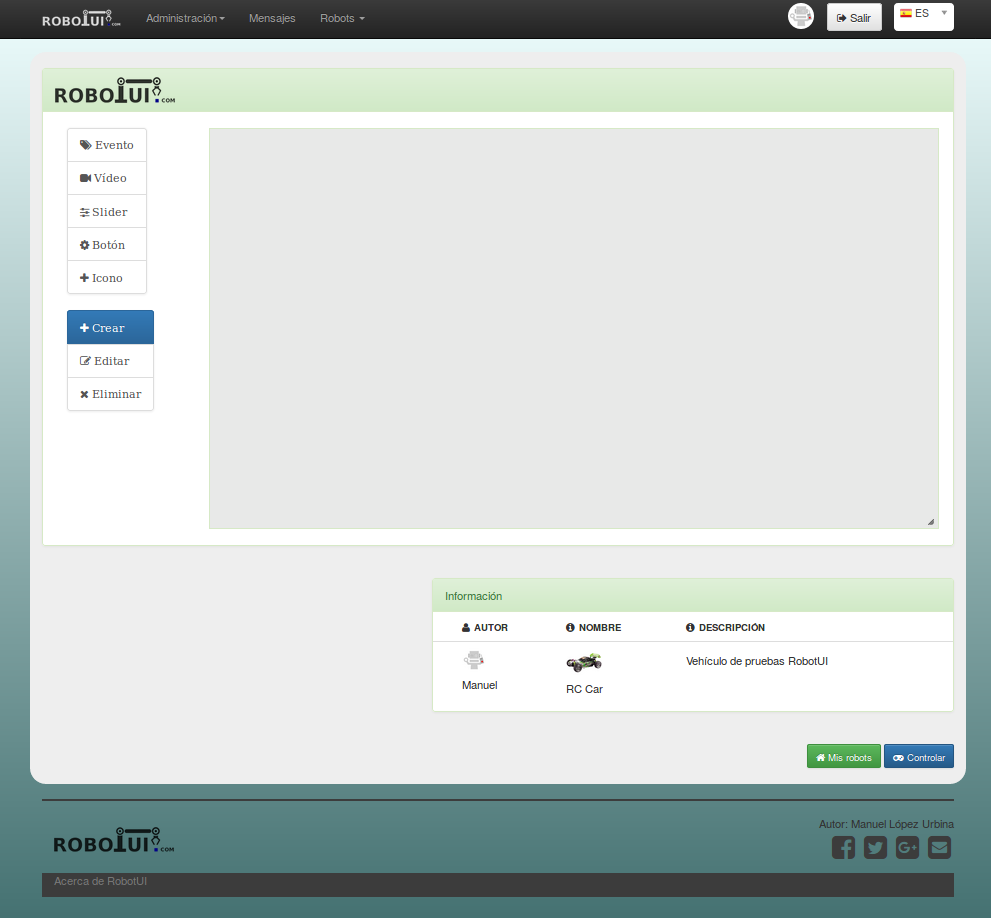
\includegraphics[scale=0.4]{imagenes/manual-usuario/pagina-configurar-interfaz.png}
  \end{center}
  \caption{Panel de configuración de la interfaz.}
  \label{website:configuracion-interfaz}
\end{figure}

La ventana de la figura \ref{website:configuracion-interfaz} se pueden apreciar los siguientes elementos:

\begin{enumerate}
  \item Panel de elementos (Evento, vídeo, Slider, Botón e Icono).
 \item Panel de acciones (Crear, editar y eliminar).
 \item Panel interfaz.
 \item Panel informativo de las características del robot.
\end{enumerate}


\begin{figure}[H]
  \begin{center}
    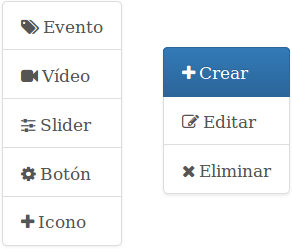
\includegraphics[scale=.6]{imagenes/manual-usuario/barra-herramientas-interfaz.png}
  \end{center}
  \caption{Panel de herramientas  y panel de acciones para la configuración de la interfaz.}
  \label{website:pagina-principal}
\end{figure}


\begin{table}[H]
  \begin{center}
    \begin{tabular}{|p{2cm}|p{10cm}|}
      \hline
      \centering{Botón} & \qquad \quad Significado \\
      \hline
      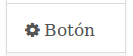
\includegraphics[width=2cm]{imagenes/manual-usuario/nuevo-boton.png} & Apertura del formulario para la creación de un botón. \\
      \hline
      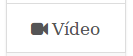
\includegraphics[width=2cm]{imagenes/manual-usuario/nuevo-video.png} & Apertura del formulario para la creación de un canvas de vídeo. \\
      \hline
      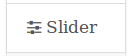
\includegraphics[width=2cm]{imagenes/manual-usuario/nuevo-slider.png} & Apertura del formulario para la creación de un slider. \\
      \hline
      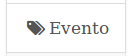
\includegraphics[width=2cm]{imagenes/manual-usuario/nuevo-evento.png} & Apertura del formulario para la creación de una etiqueta. \\
      \hline
      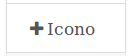
\includegraphics[width=2cm]{imagenes/manual-usuario/nuevo-icono.png} & Apertura del formulario para la subida de un icono. \\
      \hline
    \end{tabular}
  \end{center}
\caption{Elementos de una interfaz.}
\end{table}


\section{ Programa tu robot }
\label{sec:programacion-robot}

NOTA: Esta guía comprende una serie de pasos para realizar la programación de un dispositivo robótico para la aplicación RobotUI que emplee como base una placa Raspberry Pi, ya que se hace uso de su sistema de Entrada/Salio Gpio. 
El sistema es compatible con cualquier dispositivo solo que se deberán emplear a nivel de programación las librerías adecuadas para activar las salidas correspondientes al modelo de placa utilizado.\\


Para realizar la programación de nuestro dispositivo robótico debemos seguir una serie de pasos. Primero, al crear nuestro robot en la aplicación RobotUI como queda descrito en el punto \ref{sec:creacion-robot}
}, y tomando nota del identificador único que la aplicación proporciona para dicho robot.\\	

\begin{figure}[H]
  \begin{center}
    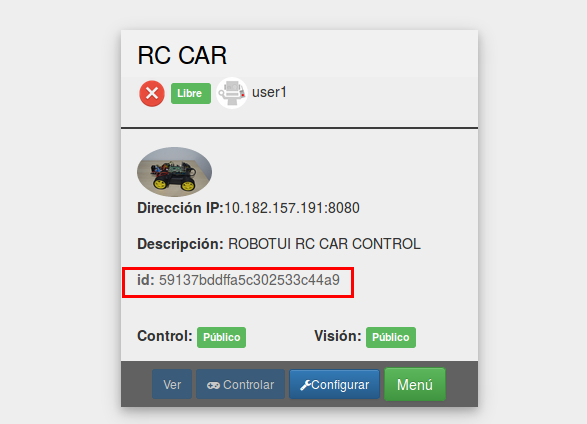
\includegraphics[scale=.6]{imagenes/manual-usuario/identificador.png}
  \end{center}
  \caption{Panel informativo del robot donde se aprecia su identificador.}
  \label{website:pagina-principal}
\end{figure}


Pasos:

\begin{enumerate}
  \item Generar una archivo con nombre client.js, por ejemplo, con el código base mostrado en el inferior.
  \item Reemplazar en el código la palabra \emph{IDENTIFICADOR} por el identificador de nuestro robot indicado en la vista show del mismo. Por ejemplo: 59188631c8e94ba54f7a4bdc
  \item Indicar el puerto en el que el rebot permanecerá a la escucha. Para ello debemos reemplazar palabra \emph{PUERTO} del código inferior por el puerto deseado. Por ejemplo 8085. 
  \item El siguiente paso es es
\end{enumerate}




\begin{lstlisting}[language=JavaScript]
var io_client = require('./node_modules/socket.io-client');
var sails_client = require('./node_modules/sails.io.js');
var io_server = sails_client(io_client);
// io.sails.url = 'http://46.101.102.33:80';
io_server.sails.url = 'http://localhost:1337';
io_server.socket.get('/robot/changetoonline/', {robot: 'IDENTIFICADOR', online: true});

// Inicia servidor socket.io en el puerto PUERTO.
var io =io_client.listen( PUERTO, { log: false });

// Carga de módulos necesarios.
var ffmpeg_command, running_camera = false, child_process = require('child_process');

var Gpio = require('pigpio').Gpio;
// Pines utilizados. Motores izquierdos: 2 y 3, motores derechos: 17 y 27
var gpio2 = new Gpio(2, {mode: Gpio.OUTPUT}),
  gpio3 = new Gpio(3, {mode: Gpio.OUTPUT}),
  gpio17 = new Gpio(17, {mode: Gpio.OUTPUT}),
  gpio27 = new Gpio(27, {mode: Gpio.OUTPUT});


console.log('Esperando conexión...');

var sockets = {};

io.sockets.on('connection', function (socket)
{

  sockets[socket.id] = socket;
  console.log("Clientes totales conectados: ", Object.keys(sockets).length);

  socket.on('disconnect', function() {
    console.log('¡Adios!');
    //stopStreaming(socket);
  });


  socket.on('start-stream', function() {
    startStreaming(socket);
  });

  socket.emit('robotmsg', {msg: "¡¡¡Bienvenido!!!"});
  console.log('emitiendo: ' + "¡¡¡Bienvenido!!!");

  socket.on('action', function (data){

    console.log('Comando recibido: ' + data);

    switch(data) {
      case 'UP':
        gpio2.digitalWrite(1);
        gpio3.digitalWrite(0);
        gpio17.digitalWrite(1);
        gpio27.digitalWrite(0);
        console.log('UP');
        break;

      case 'RIGHT':
        gpio2.digitalWrite(0);
        gpio3.digitalWrite(0);
        gpio17.digitalWrite(1);
        gpio27.digitalWrite(0);
        console.log('UP');
        break;

      case 'LEFT':
        gpio2.digitalWrite(1);
        gpio3.digitalWrite(0);
        gpio17.digitalWrite(0);
        gpio27.digitalWrite(0);
        console.log('UP');
        break;

      case 'DOWN':
        gpio2.digitalWrite(0);
        gpio3.digitalWrite(1);
        gpio17.digitalWrite(0);
        gpio27.digitalWrite(1);
        console.log('UP');
        break;

      case 'STOP':
        gpio2.digitalWrite(0);
        gpio3.digitalWrite(0);
        gpio17.digitalWrite(0);
        gpio27.digitalWrite(0);
        console.log('UP');
        break;

      default:
        console.log('command not found');
    }

  })
});

function stopStreaming(socket) {
  delete sockets[socket.id];
  // no more sockets, kill the stream
  if (Object.keys(sockets).length == 0) {
    if (ffmpeg_command){
      ffmpeg_command.kill();
      running_camera = false;
      console.log('Stop streaming');
    }
  }
}

function startStreaming(socket) {
  //ffmpeg -f video4linux2 -i /dev/video0 -s 300x150 -f mjpeg pipe:1 -b:v 28k -bufsize 28k

  if (running_camera == false){
    console.log('Starting streaming....');
    var args = ["-f", "video4linux2", "-i", "/dev/video0", "-s", "300x150","-f","mjpeg", "pipe:1", "-b:v 28k", "-bufsize 28k"]
    ffmpeg_command = child_process.spawn("ffmpeg", args);
    running_camera = true
  }

  ffmpeg_command.on('error', function(err, stdout, stderr) {
    console.log("ffmpeg stdout:\n" + stdout);
    console.log("ffmpeg stderr:\n" + stderr);
    running_camera = false
  });


  ffmpeg_command.on('close', function (code) {
    console.log('ffmpeg exited' + code );
    running_camera = false
  });


  ffmpeg_command.stderr.on('data', function (data) {
    //console.log('stderr: ' + data);
  });

  ffmpeg_command.on('end', function() {
    console.log('Fin');
    running_camera = false
  });

  ffmpeg_command.stdout.on('data', function (data) {
    //console.log('stdout: ' + data);
    var frame = new Buffer(data).toString('base64');
    socket.emit('canvas',frame);
  });

}

\end{lstlisting}

Una vez generado el código debemos copiarlo a la placa Raspberry Pi o computador que actuará como Robot para nuestra aplicación y ejecutarlo. Para la ejecución del código introducimos el siguiente comando:\\

\begin{lstlisting}[language=bash]
  sudo node raspberry.js
\end{lstlisting}

Siendo \emph{raspberry.js} el nombre del archivo que contiene nuestro código.


\section{ Controla tu robot }
\label{sec:control-robot}

El panel de control de la interfaz podemos identificar los siguientes elementos:

\begin{figure}[H]
  \begin{center}
    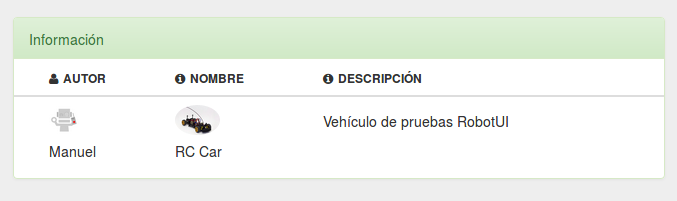
\includegraphics[scale=.6]{imagenes/manual-usuario/panel-robot-info.png}
  \end{center}
  \caption{ Panel informativo de las características del robot de la interfaz.}
  \label{website:pagina-principal}
\end{figure}


\begin{figure}[H]
  \begin{center}
    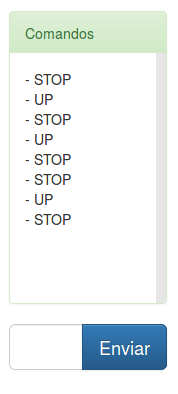
\includegraphics[scale=.6]{imagenes/manual-usuario/panel-comandos.png}
  \end{center}
  \caption{ Panel informativo de las órdenes enviadas al robot junto con una entrada de comandos para enviar nuevas órdenes directamente.}
  \label{website:pagina-principal}
\end{figure}


\section{ Visita otros robots }
\label{sec:visita-robot}


